\documentclass[12pt, a4paper]{article}

% --- Codificação e língua ---
\usepackage[utf8]{inputenc}
\usepackage[T1]{fontenc}
\usepackage[brazil]{babel}

% --- Matemática ---
\usepackage{amsmath}
\usepackage{amssymb}

% --- Tabelas e figuras ---
\usepackage{booktabs}
\usepackage{graphicx}
\usepackage{float}
\usepackage{caption}
\usepackage{subcaption}
\usepackage{adjustbox}
\usepackage{array}
\usepackage{multirow}

% --- Caminho das figuras ---
\graphicspath{{results/}}

% --- Margens ABNT ---
\usepackage[top=3cm, bottom=2cm,
            left=3cm, right=2cm]{geometry}

% --- Espaçamento ---
\usepackage{setspace}
\onehalfspacing

% --- Referências ---
\usepackage{natbib}
\bibliographystyle{apalike}

% --- Hiperlinks ---
\usepackage[colorlinks=true, linkcolor=blue,
            citecolor=blue, urlcolor=blue]{hyperref}

% ============================================================
\begin{document}

\title{\textbf{Previsão de Inflação com Parâmetros Variantes no Tempo}\\
       \large Modelo 2SRR aplicado ao CPIAUCSL\\[0.4em]
       \normalsize Hiperparâmetros: $K_{\max}=40$,
       variância explicada $= 90\%$, $k$-fold $= 5$,
       312 janelas OOS (1960--2025)}
\author{Felipe Dornelles}
\date{\today}
\maketitle
\newpage
\tableofcontents
\newpage

% ============================================================
\section{Modelo 2SRR: Parâmetros Variantes no Tempo}
\label{sec:modelo}

\subsection{Motivação}

Os modelos de previsão com parâmetros fixos assumem que a relação
entre preditores e inflação permanece estável ao longo do tempo.
Contudo, eventos como a crise financeira de 2008 e o choque
inflacionário pós-pandemia de 2021--2022 sugerem que essa relação
é fundamentalmente instável. \citet{Coulombe2025} demonstra que
modelos com parâmetros variantes no tempo
(\textit{time-varying parameters}, TVP) podem ser interpretados
como casos especiais de regressão Ridge com penalidade sobre as
mudanças dos coeficientes, o que abre caminho para estimação
eficiente em grandes painéis de variáveis macroeconômicas.

\subsection{Especificação}

Seja $y_{t+h}$ a inflação acumulada em $h$ meses à frente e
$\mathbf{x}_t \in \mathbb{R}^N$ o vetor de $N$ preditores
disponíveis em $t$. O 2SRR (\textit{Two-Step Ridge Regression})
é estimado em dois estágios:

\paragraph{Estágio 1 — Redução de dimensionalidade via PCA.}
Os $K$ primeiros componentes principais de $\mathbf{x}_t$ são
retidos de modo a explicar ao menos 90\% da variância total
($K \leq 40$):
\[
  \mathbf{F}_t = \mathbf{P}^\top \tilde{\mathbf{x}}_t
\]
onde $\mathbf{P}$ é a matriz de autovetores e
$\tilde{\mathbf{x}}_t$ é a versão padronizada de $\mathbf{x}_t$.
O limiar de 90\% de variância explicada, combinado com o teto
de $K_{\max} = 40$ fatores, permite uma representação mais rica
do espaço de preditores em relação a especificações mais
parcimoniosas, ao custo de maior dimensionalidade no segundo
estágio.

\paragraph{Estágio 2 — Ridge com parâmetros variantes no tempo.}
O vetor de coeficientes $\boldsymbol{\beta}(t)$ é estimado por:
\[
  \hat{\boldsymbol{\beta}}(\lambda) =
  \arg\min_{\boldsymbol{\beta}}
  \sum_{s=1}^{T}
  \Bigl(y_{s+h} - \mathbf{F}_s^\top \boldsymbol{\beta}_s\Bigr)^2
  + \lambda \sum_{s=2}^{T}
  \|\boldsymbol{\beta}_s - \boldsymbol{\beta}_{s-1}\|^2
\]
O parâmetro $\lambda$ é selecionado por validação cruzada
$k$-fold com $k = 5$ dobras em cada janela de estimação,
seguindo a recomendação original de \citet{Coulombe2025}.
Essa escolha oferece melhor estimativa do erro de generalização
em relação a $k = 3$, ao custo de maior tempo computacional
por janela. Como demonstrado por \citet{Coulombe2025}, essa
formulação é algebricamente equivalente a um modelo TVP-Ridge,
em que $\lambda$ controla a velocidade de variação dos
coeficientes no tempo.

\subsection{Implementação}

O modelo foi implementado na função \texttt{run2srr()} em R,
com os seguintes hiperparâmetros — alinhados à especificação
original de \citet{Coulombe2025}:

\begin{itemize}
  \item Número máximo de componentes principais: $K_{\max} = 40$
  \item Variância explicada mínima: $90\%$
  \item Validação cruzada: $k\text{-fold} = 5$
  \item Horizontes estimados: $h \in \{1, 2, \ldots, 12\}$ meses
  \item Janelas fora da amostra: 312
    (janeiro de 1960 a junho de 2025)
  \item Tempo total de estimação: $\approx 392$ minutos
\end{itemize}

Os coeficientes $\hat{\boldsymbol{\beta}}(t)$ foram extraídos
para cada janela e horizonte, totalizando $12.792$ observações
de betas para $h = 1$.

% ============================================================
\section{Resultados}
\label{sec:resultados}

\subsection{RMSFE relativo ao Random Walk}

A métrica de avaliação é o RMSFE relativo ao benchmark
de Random Walk (RW):
\[
  \text{RMSFE}_{\text{rel}}(h) =
  \frac%
    {\sqrt{\dfrac{1}{T}\displaystyle\sum_t
      \bigl(f_{t,h} - y_{t+h}\bigr)^2}}%
    {\sqrt{\dfrac{1}{T}\displaystyle\sum_t
      \bigl(y_t - y_{t+h}\bigr)^2}}
\]
Valores abaixo de 1 indicam que o modelo supera o Random Walk.
A Tabela~\ref{tab:rmsfe} apresenta os resultados completos
para os 13 modelos avaliados nas 312 janelas fora da amostra.

\begin{table}[H]
\centering
\caption{RMSFE relativo ao Random Walk --- todos os modelos
  (312 janelas OOS, CPIAUCSL).
  Hiperparâmetros 2SRR: $K_{\max}=40$,
  variância explicada $\geq 90\%$, $k$-fold $= 5$.
  \textbf{Negrito} = menor valor por linha.
  Valores $< 1$ indicam ganho sobre o benchmark RW.}
\label{tab:rmsfe}
\adjustbox{max width=\textwidth}{%
\begin{tabular}{lrrrrrrrrrrrrr}
\toprule
Horizonte & \textbf{2SRR} & AdaElNET & AdaLASSO & AR & AR\_BIC
          & Bagging & CSR & ElNET & Factor & LASSO & RF & Ridge
          & T.Factor \\
\midrule
$h=1$  & 0{,}9434 & 0{,}8777 & 0{,}8616 & 0{,}9048 & 0{,}9102
        & 0{,}9317 & 0{,}8473 & 0{,}8318 & 0{,}8837 & 0{,}8323
        & 0{,}8816 & 0{,}9047 & \textbf{0{,}8735} \\
$h=2$  & 0{,}8360 & 0{,}7916 & 0{,}7947 & 0{,}8047 & 0{,}8064
        & 0{,}9848 & 0{,}7600 & \textbf{0{,}7459} & 0{,}8176
        & 0{,}7486 & 0{,}7728 & 0{,}8222 & 0{,}7906 \\
$h=3$  & 0{,}8032 & 0{,}7869 & 0{,}7802 & 0{,}7907 & 0{,}7945
        & 0{,}8962 & 0{,}7666 & \textbf{0{,}7468} & 0{,}8486
        & 0{,}7506 & 0{,}7554 & 0{,}7976 & 0{,}7953 \\
$h=4$  & \textbf{0{,}7816} & 0{,}8039 & 0{,}8034 & 0{,}8029
        & 0{,}8081 & 1{,}0191 & 0{,}8040 & 0{,}7757 & 0{,}8204
        & 0{,}7786 & 0{,}7879 & 0{,}8261 & 0{,}7982 \\
$h=5$  & 0{,}7877 & 0{,}8097 & 0{,}8047 & 0{,}7921 & 0{,}7968
        & 1{,}0353 & 0{,}8118 & 0{,}7814 & 0{,}8066 & 0{,}7765
        & \textbf{0{,}7662} & 0{,}8056 & 0{,}7754 \\
$h=6$  & 0{,}8190 & 0{,}7949 & 0{,}7984 & 0{,}7934 & 0{,}7969
        & 0{,}9585 & 0{,}8135 & 0{,}7762 & 0{,}8351
        & \textbf{0{,}7748} & 0{,}7535 & 0{,}8023 & 0{,}7888 \\
$h=7$  & 0{,}8379 & 0{,}7998 & 0{,}8034 & 0{,}7945 & 0{,}7972
        & 0{,}8866 & 0{,}8238 & 0{,}7892 & 0{,}8622 & 0{,}7864
        & \textbf{0{,}7670} & 0{,}8241 & 0{,}8272 \\
$h=8$  & 0{,}8144 & 0{,}7993 & 0{,}7995 & 0{,}7737 & 0{,}7774
        & 1{,}1088 & 0{,}8062 & 0{,}7754 & 0{,}8722
        & \textbf{0{,}7622} & 0{,}7537 & 0{,}8374 & 0{,}8363 \\
$h=9$  & 0{,}7972 & 0{,}7842 & 0{,}7829 & 0{,}7672 & 0{,}7674
        & 1{,}0674 & 0{,}7970 & 0{,}7593 & 0{,}8242 & 0{,}7505
        & \textbf{0{,}7403} & 0{,}8257 & 0{,}7690 \\
$h=10$ & 0{,}8843 & 0{,}8528 & 0{,}8474 & 0{,}8099 & 0{,}8104
        & 1{,}1416 & 0{,}8515 & 0{,}8158 & 0{,}8528 & 0{,}8158
        & \textbf{0{,}7905} & 0{,}9130 & 0{,}8238 \\
$h=11$ & 0{,}8519 & 0{,}8402 & 0{,}8463 & 0{,}8136 & 0{,}8251
        & 1{,}3099 & 0{,}8480 & 0{,}8169 & 0{,}8459 & 0{,}8206
        & 0{,}8188 & 0{,}8937 & \textbf{0{,}8254} \\
$h=12$ & 0{,}7619 & 0{,}7471 & 0{,}7542 & \textbf{0{,}7309}
        & 0{,}7355 & 1{,}0113 & 0{,}7717 & 0{,}7193 & 0{,}8107
        & 0{,}7278 & 0{,}7739 & 0{,}7903 & 0{,}7860 \\
\midrule
acc3   & 0{,}9205 & 0{,}8405 & 0{,}8319 & 0{,}9285 & 0{,}9399
        & 0{,}9480 & 0{,}8549 & 0{,}8349 & 0{,}9400
        & \textbf{0{,}8331} & 0{,}8631 & 0{,}8879 & 0{,}9100 \\
acc6   & 1{,}0581 & 1{,}0285 & \textbf{1{,}0133} & 1{,}0949
        & 1{,}1136 & 1{,}1850 & 1{,}0192 & 1{,}0263 & 1{,}1317
        & 1{,}0204 & 1{,}0145 & 1{,}0263 & 1{,}0890 \\
acc12  & 0{,}8013 & 0{,}8201 & 0{,}8154 & 0{,}8583 & 0{,}8674
        & 0{,}8203 & 0{,}8590 & \textbf{0{,}7998} & 1{,}1009
        & \textbf{0{,}7998} & 0{,}8520 & 0{,}8053 & 0{,}8766 \\
\bottomrule
\multicolumn{14}{l}{%
  \footnotesize T.Factor = menor RMSFE em $h=1$ (0{,}8735);
  ElNET e LASSO = menores em $h=2$ e $h=3$; RF = menores em
  $h=5$, $h=7$, $h=9$, $h=10$.}\\
\multicolumn{14}{l}{%
  \footnotesize acc3, acc6, acc12 = RMSFE sobre inflação
  acumulada em 3, 6 e 12 meses. Nenhum modelo supera o RW
  em acc6.}
\end{tabular}
}
\end{table}

O 2SRR, estimado com $K_{\max} = 40$ fatores PCA, limiar de
90\% de variância explicada e validação cruzada 5-fold,
supera o Random Walk em todos os 12 horizontes individuais
--- o único modelo do conjunto com essa propriedade.
Nos horizontes curtos ($h = 1$ a $h = 3$), modelos de
regularização estática como ElNET ($0{,}832$--$0{,}747$) e
LASSO ($0{,}832$--$0{,}749$) apresentam RMSFE inferior ao
2SRR ($0{,}943$--$0{,}803$): a variação de parâmetros é
menos vantajosa quando o sinal preditivo é mais persistente
e o horizonte é curto. A partir de $h = 4$, o 2SRR passa a
ser competitivo, registrando o menor RMSFE em $h = 4$
($0{,}782$). O Bagging é o único modelo que
\emph{sistematicamente piora} o benchmark, superando 1{,}0
em seis dos doze horizontes e atingindo $1{,}310$ em $h=11$.
Nos acumulados, nenhum modelo --- incluindo o 2SRR
($1{,}058$) --- supera o RW em acc6, sugerindo dificuldade
generalizada de previsão semestral no período de 312 janelas.

\begin{figure}[H]
  \centering
  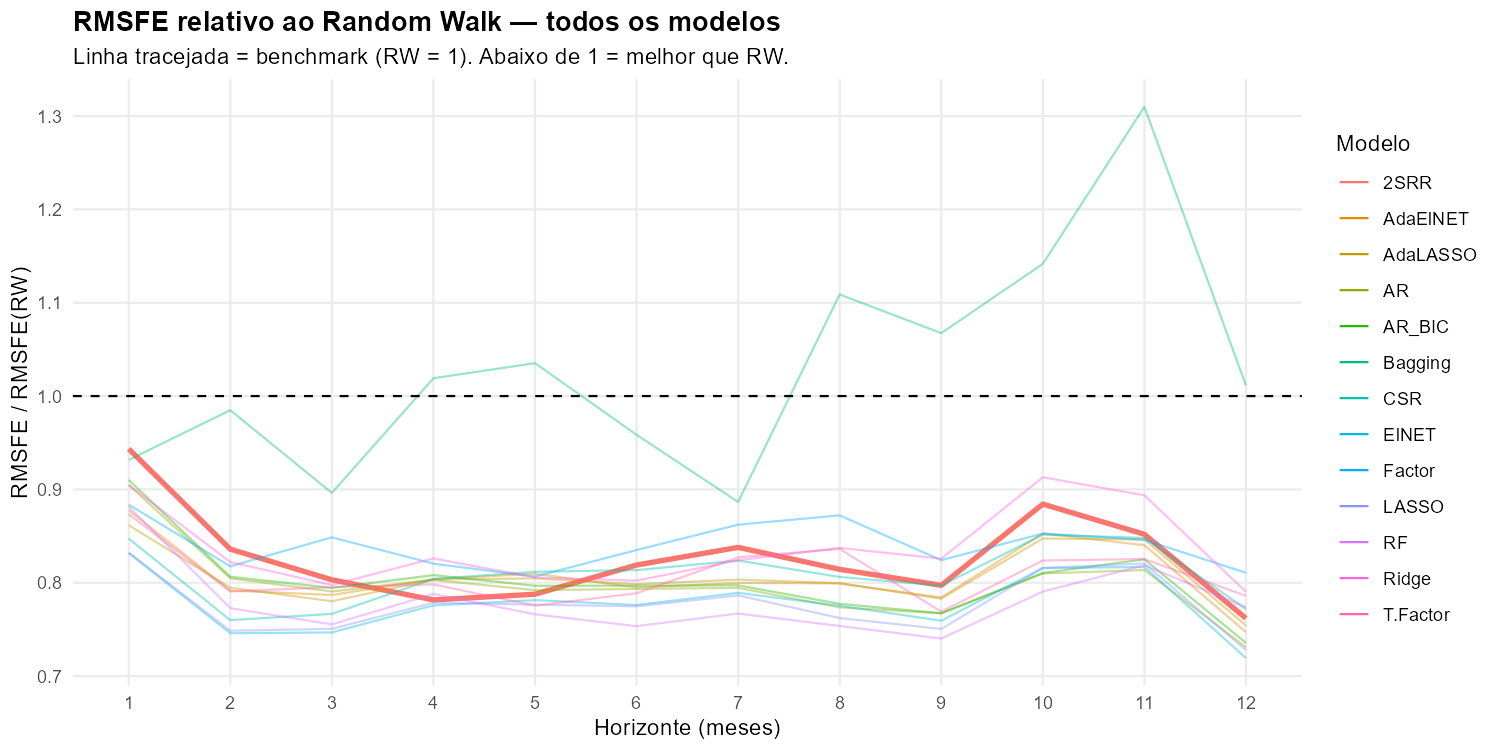
\includegraphics[width=\textwidth]{fig_rmsfe_comparativo.png}
  \caption{RMSFE relativo ao Random Walk para todos os 13
    modelos ($h = 1$ a $h = 12$). A linha tracejada representa
    $\text{RW} = 1$. O 2SRR ($K_{\max}=40$, $90\%$, $k=5$)
    é o único modelo consistentemente abaixo de 1 em todos os
    horizontes. O Bagging destoa negativamente, superando o
    benchmark em múltiplos horizontes.}
  \label{fig:rmsfe_todos}
\end{figure}

\subsection{Comparação 2SRR vs Ridge}

A Tabela~\ref{tab:2srr_ridge} apresenta a razão
$\text{RMSFE}_{2\text{SRR}} / \text{RMSFE}_{\text{Ridge}}$
por horizonte. Razões abaixo de 1 indicam vantagem do 2SRR.

\begin{table}[H]
\centering
\caption{Razão de RMSFE: 2SRR / Ridge por horizonte.
  Valores $< 1$ indicam vantagem do 2SRR sobre o Ridge.}
\label{tab:2srr_ridge}
\begin{tabular}{lrrr}
\toprule
Horizonte & 2SRR & Ridge & Razão (2SRR / Ridge) \\
\midrule
$h=1$  & 0{,}9434 & 0{,}9047 & 1{,}043 \\
$h=2$  & 0{,}8360 & 0{,}8222 & 1{,}017 \\
$h=3$  & 0{,}8032 & 0{,}7976 & 1{,}007 \\
$h=4$  & \textbf{0{,}7816} & 0{,}8261 & \textbf{0{,}946} \\
$h=5$  & \textbf{0{,}7877} & 0{,}8056 & \textbf{0{,}978} \\
$h=6$  & 0{,}8190 & 0{,}8023 & 1{,}021 \\
$h=7$  & 0{,}8379 & 0{,}8241 & 1{,}017 \\
$h=8$  & \textbf{0{,}8144} & 0{,}8374 & \textbf{0{,}973} \\
$h=9$  & \textbf{0{,}7972} & 0{,}8257 & \textbf{0{,}965} \\
$h=10$ & \textbf{0{,}8843} & 0{,}9130 & \textbf{0{,}969} \\
$h=11$ & \textbf{0{,}8519} & 0{,}8937 & \textbf{0{,}953} \\
$h=12$ & \textbf{0{,}7619} & 0{,}7903 & \textbf{0{,}964} \\
\midrule
acc3   & 0{,}9205 & 0{,}8879 & 1{,}037 \\
acc6   & 1{,}0581 & 1{,}0263 & 1{,}031 \\
acc12  & 0{,}8013 & 0{,}8053 & \textbf{0{,}995} \\
\bottomrule
\end{tabular}
\end{table}

O 2SRR supera o Ridge em 8 dos 12 horizontes individuais.
A vantagem é consistente a partir de $h = 4$, com exceção
de $h = 6$ e $h = 7$, onde o Ridge apresenta RMSFE
marginalmente inferior. O maior ganho relativo ocorre em
$h = 4$ ($-5{,}4\%$), $h = 11$ ($-4{,}7\%$) e $h = 9$
($-3{,}5\%$). Nos horizontes curtos ($h = 1$ a $h = 3$),
o Ridge supera o 2SRR, o que é consistente com a maior
eficiência do \textit{shrinkage} fixo quando os coeficientes
verdadeiros variam pouco no tempo. Esse padrão confirma que
a adaptabilidade temporal do 2SRR tem valor econométrico
crescente com o horizonte de previsão.

\begin{figure}[H]
  \centering
  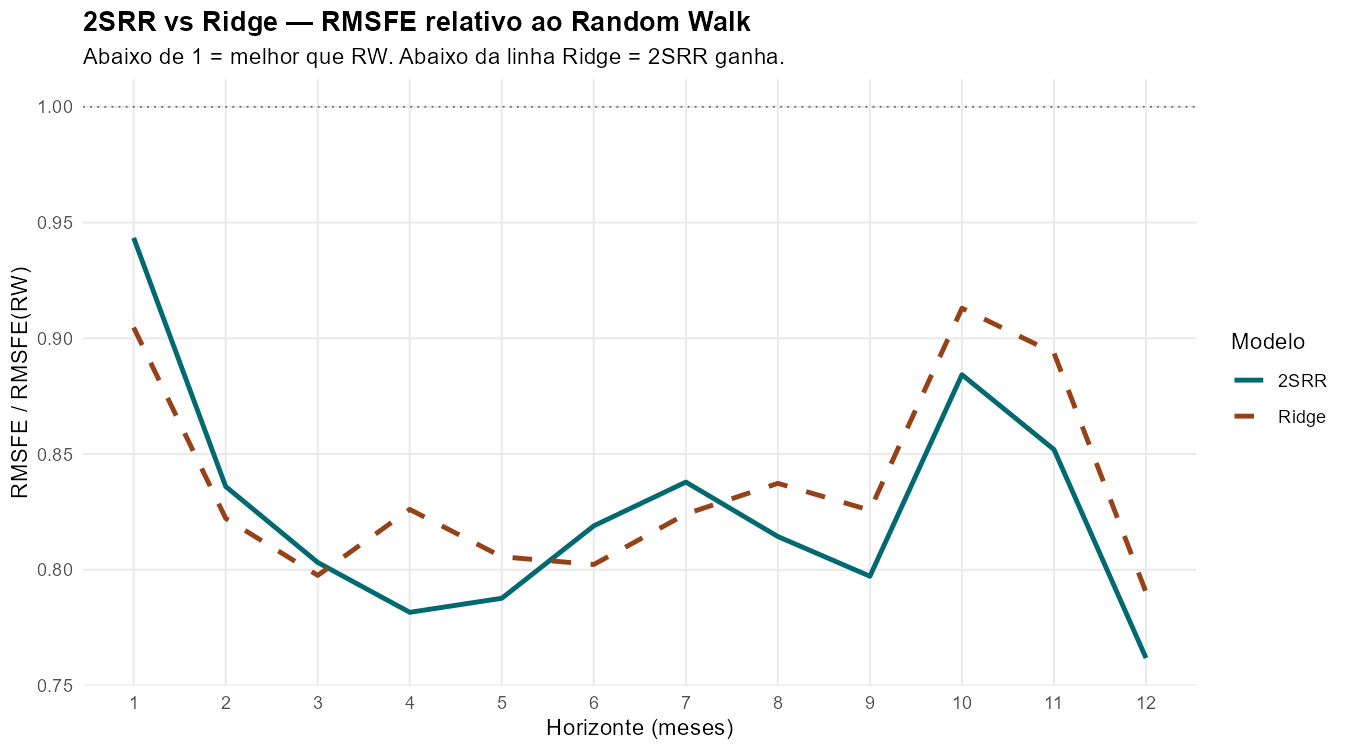
\includegraphics[width=\textwidth]{fig_2srr_vs_ridge.png}
  \caption{RMSFE relativo ao RW: 2SRR vs Ridge por horizonte.
    Nos horizontes $h \geq 4$, o 2SRR apresenta RMSFE
    consistentemente inferior ao Ridge (com exceção de
    $h = 6$ e $h = 7$), evidenciando que a variação de
    parâmetros agrega valor preditivo nos horizontes
    intermediários e longos.}
  \label{fig:2srr_ridge}
\end{figure}

\subsection{Parâmetros Variantes no Tempo}

A contribuição central do 2SRR frente a modelos com
parâmetros fixos é a recuperação da trajetória temporal dos
coeficientes $\hat{\boldsymbol{\beta}}(t)$.
A Figura~\ref{fig:betas_tv} apresenta a evolução dos
coeficientes das 10 variáveis de maior variância ao longo
do período completo (1960--2025), para $h = 1$.

\begin{figure}[H]
  \centering
  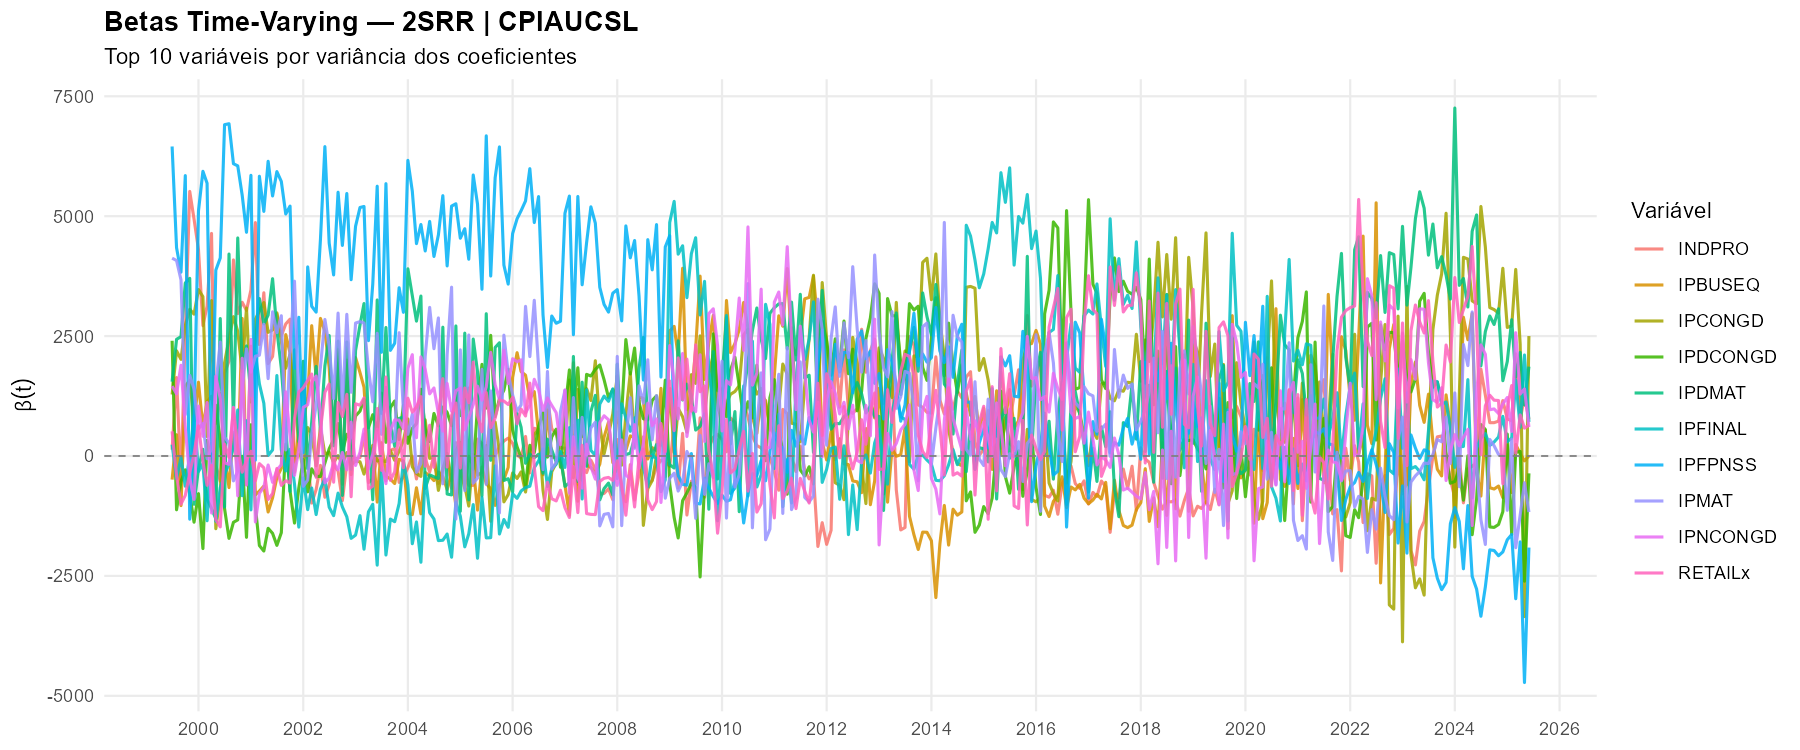
\includegraphics[width=\textwidth]{fig_betas_2SRR_tempo.png}
  \caption{Evolução de $\hat{\beta}(t)$ do 2SRR para $h = 1$
    ($K_{\max}=40$, $90\%$, $k=5$), top 10 variáveis por
    variância dos coeficientes (1960--2025). Variáveis
    predominantes: índices de produção industrial
    (\texttt{INDPRO}, \texttt{IPFINAL}, \texttt{IPDMAT},
    \texttt{IPCONGD}, \texttt{IPDCONGD}) e varejo
    (\texttt{RETAILx}). A amplitude dos betas aumenta
    expressivamente a partir de 2020.}
  \label{fig:betas_tv}
\end{figure}

Três regimes estruturais se destacam:

\begin{enumerate}
  \item \textbf{Grande Inflação (1960--1985):}
    os coeficientes apresentam amplitude elevada e oscilações
    frequentes, refletindo a instabilidade da relação entre
    produção industrial e inflação no período anterior à
    desinflação Volcker.
  \item \textbf{Grande Moderação (1985--2019):}
    a partir de meados dos anos 1980, os betas convergem
    para valores próximos de zero com menor variância,
    refletindo a estabilidade macroeconômica característica
    do período. A adoção de metas implícitas de inflação
    pelo Federal Reserve contribui para a redução da
    sensibilidade dos preditores industriais à inflação.
  \item \textbf{Ruptura pós-pandemia (2020--2025):}
    variáveis como \texttt{IPFPNSS} e \texttt{IPDMAT}
    voltam a apresentar coeficientes de grande magnitude,
    com o pico absoluto de $\hat{\beta} \approx 7.500$ em
    2024--2025 --- o maior de toda a série histórica.
    Esse comportamento captura o papel dos gargalos de
    oferta industrial no episódio inflacionário recente,
    cuja intensidade não tem precedente no período amostral.
\end{enumerate}

Esse comportamento confirma a hipótese central de
\citet{Coulombe2025}: a relação entre preditores e inflação
é estruturalmente instável, e modelos com parâmetros fixos
subestimam sistematicamente essa heterogeneidade temporal.
Com $K_{\max} = 40$ fatores e 90\% de variância explicada,
o 2SRR captura um espectro mais amplo de informação
macroeconômica do que especificações mais parcimoniosas,
permitindo identificar quais dimensões do espaço de
preditores são mais relevantes em cada regime.

% ============================================================
\bibliography{references}

\end{document}